% This is samplepaper.tex, a sample chapter demonstrating the
% LLNCS macro package for Springer Computer Science proceedings;
% Version 2.21 of 2022/01/12
%
\documentclass[runningheads]{llncs}
%
\usepackage[T1]{fontenc}
% T1 fonts will be used to generate the final print and online PDFs,
% so please use T1 fonts in your manuscript whenever possible.
% Other font encondings may result in incorrect characters.
%
\usepackage{graphicx}
% Used for displaying a sample figure. If possible, figure files should
% be included in EPS format.
%
% If you use the hyperref package, please uncomment the following two lines
% to display URLs in blue roman font according to Springer's eBook style:
% \usepackage{color}
% \renewcommand\UrlFont{\color{blue}\rmfamily}
%
\usepackage{hyperref}
\usepackage{paralist}
\usepackage{booktabs}
\usepackage{totcount}
\usepackage{amssymb}

\newcounter{totHours} %to track the estimate of total hours to assess SOP
\setcounter{totHours}{0}
\regtotcounter{totHours}

\newcounter{rqnum} %research question number
\newcommand{\rqtherqnum}{RQ`'\therqnum}
\newcommand{\rqref}[1]{RQ\ref{#1}}

\newcounter{pnum} %pain point number
\newcommand{\ppthepnum}{P`'\thepnum}
\newcommand{\ppref}[1]{P\ref{#1}}

\newcommand{\CC}{C\nolinebreak\hspace{-.05em}\raisebox{.4ex}{\small\bf
+}\nolinebreak\hspace{-.10em}\raisebox{.4ex}{\small\bf +}}

\begin{document}
%
% \title{Digging Deep to Assess the State of the Practice for Different Research Software Domains}
\title{Digging Deeper Into the State of the Practice for Domain Specific Research Software}
\titlerunning{Digging Deeper}
% If the paper title is too long for the running head, you can set
% an abbreviated paper title here
%
\author{Spencer Smith\inst{1}\orcidID{0000-0002-0760-0987} \and
Peter Michalski\inst{1}}%\orcidID{1111-2222-3333-4444} \and
%Third Author\inst{3}\orcidID{2222--3333-4444-5555}}
%
\authorrunning{S.\ Smith and P.\ Michalski}
% First names are abbreviated in the running head.
% If there are more than two authors, 'et al.' is used.
%
\institute{McMaster University, 1280 Main Street West, Hamilton ON L8S 4K1, Canada
\email{smiths@mcmaster.ca}\\
\url{http://www.cas.mcmaster.ca/~smiths/}}
%
\maketitle % typeset the header of the contribution
%
\begin{abstract}

	We have developed a methodology for assessing the state of the software
	development practice for a given research software domain. Our methodology
	prescribes the following steps: i) Identify the domain; ii) Identify a list
	of candidate software packages; iii) Filter the list to a length of about 30
	packages; iv) Collect repository related data on each software package, like
	number of stars, number of open issues, number of lines of code; v) Fill in
	the measurement template (the template consists of 108 questions to assess 9
	qualities (including the qualities of installability, usability and
	visibility)); vi) Rank the software using the Analytic Hierarchy Process
	(AHP); vii) Interview developers (the interview consists of 20 questions and
	takes about an hour); and, viii) Conduct a domain analysis. The collected
	data is analyzed by: i) comparing the ranking by best practices against 
	the ranking by popularity; ii) comparing artifacts, tools and processes to
	current research software development guidelines; and, iii) exploring pain
	points. We estimate the time to complete an assessment for a given domain at
	173 person hours. The method is illustrated via the example of Lattice
	Boltzmann Solvers, where we find that the top packages engaged in most of
	recommended best practices, but still show room for improvement with respect
	to providing API documentation, a roadmap, a code of conduct, programming
	style guide, uninstall instructions and continuous integration.

\keywords{research software \and software quality \and empirical measures \and analytic hierarchy process \and software artifacts \and developer pain points \and Lattice Boltzmann Method}

\end{abstract}

\section{Introduction} \label{SecIntroduction}

Research software is critical for tackling problems in areas as diverse as
manufacturing, financial planning, environmental policy and medical diagnosis
and treatment.  However, developing reliable, reproducible, sustainable and fast
research software to address new problems is challenging because of the
complexity of the physical models and the nuances of floating point and parallel
computation. The importance of research software and the difficulty with its
development have prompted multiple researchers to investigate how developing
this software differs from other classes of software.  Previous studies have
focused on surveying developers
\cite{HannayEtAl2009,Nguyen-HoanEtAl2010,PintoEtAl2018}, developer interviews
\cite{Kelly2013} and case studies \cite{CarverEtAl2007,Segal2005}.  A
valuable source of information that has received less attention is the data in
publicly available software repositories.  We propose digging deeper into how
well projects are applying best practices by using a new methodology that
combines manual and automated techniques to extract repository-based
information.

The surveys used in previous studies have tended to recruit participants from
all domains of research software, possibly distinguishing them by programming
language (for instance, R developers~\cite{PintoEtAl2018}), or by the role of
the developers (for instance postdoctoral researchers \cite{UditAndKatz2017}).
Case studies, on the other hand, have focused on a few specific examples at a
time, as is the nature of case studies.  For our new methodology, we propose a
scope between these two extremes.  Rather than focus on all research software,
or just a few examples, we will focus on one domain at a time. The practical
reason for this scope is that digging deep takes time, making a broad scope
infeasible. We have imposed a practical constraint of one person month of effort
per domain.\footnote{A person month is considered to be $20$ working days ($4$
weeks in a month, with $5$ days of work per week) at $8$ person hours per day,
or $20 \cdot 8 = 160$ person hours.} Focusing on one domain at a time has more
than just practical advantages.  By restricting ourselves to a single domain we
can bring domain knowledge and domain experts into the mix.  The domain
customized insight provided by the assessment has the potential to help a
specific domain as they adopt and develop new practices.  Moreover, measuring
multiple different domains facilitates comparing and contrasting domain specific
practices.

Our methodology is built around 10 research questions.  Assuming that the domain
has been identified (Section~\ref{SecIdentifyDomain}), the first question is:

\begin{enumerate}
	\item[RQ\refstepcounter{rqnum}\therqnum \label{RQ_WhatProjects}:] What
	software projects exist in the domain, with the constraint that the source
	code must be available for all identified projects?
	(Sections~\ref{identifysoftware},~\ref{filtersoftware})
\end{enumerate}

We next wish to assess the representative software to determine how well they
apply current software development best practices.  At this point in the
process, to remove potential user/developer bias, we will base our assessment
only on publicly available artifacts, where artifacts are the documents, scripts
and code that we find in a project's public repository. Example artifacts
include requirements, specifications, user manuals, unit test cases, system
tests, usability tests, build scripts, API (Application Programming Interface)
documentation, READMEs, license documents, process documents, and code.
Following best practices does not guarantee popularity, so we will also compare
our ranking to how the user community itself ranks the identified projects.

\begin{enumerate}
	\item [RQ\refstepcounter{rqnum}\therqnum \label{RQ_HighestQuality}:] Which
	of the projects identified in \rqref{RQ_WhatProjects} follow current best
	practices, based on evidence found by experimenting with the software and
	searching the artifacts available in each project's repository? (Sections~\ref{empiricalmeasures})
	\item [RQ\refstepcounter{rqnum}\therqnum \label{RQ_CompareHQ2Popular}:] How
	similar is the list of top projects identified in \rqref{RQ_HighestQuality}
	to the most popular projects, as viewed by the scientific community? (Section~\ref{repmetrics})
\end{enumerate}

To understand the state of the practice we wish to learn the frequency with
which different artifacts appear, the types of development tools used and the
methodologies used for software development.  With this data, we can ask
questions about how the domain software compares to other research software.

\begin{enumerate}
  \item [RQ\refstepcounter{rqnum}\therqnum \label{RQ_CompareArtifacts}:] How
	do domain projects compare to research software in general with respect to the
	artifacts present in their repositories? (Section~\ref{Sec_CompareArtifacts})
	\item [RQ\refstepcounter{rqnum}\therqnum \label{RQ_CompareToolsProjMngmnt}:]
	How do domain projects compare to research software in general with respect to
	the use of tools (Section~\ref{Sec_CompareTools}) for:
	\begin{enumerate} 
		\item [\rqref{RQ_CompareToolsProjMngmnt}.a] development; and,
		\item [\rqref{RQ_CompareToolsProjMngmnt}.b] project management?
	\end{enumerate}
	\item [RQ\refstepcounter{rqnum}\therqnum \label{RQ_CompareMethodologies}:]
	How do domain projects compare to research software in general with respect to
	the processes used? (Section~\ref{Sec_CompareMethodologies})
\end{enumerate}	

Only so much information can be gleaned by digging into software repos.
To gain additional insight, we need to interview developers
(Section~\ref{SecSurvey}) to learn:

\begin{enumerate}
	\item [RQ\refstepcounter{rqnum}\therqnum \label{RQ_PainPoints}:] What are
	the pain points for developers working on domain software projects?
	(Section~\ref{painpoints})
	\item [RQ\refstepcounter{rqnum}\therqnum \label{RQ_ComparePainPoints}:] How
	do the pain points of domain developers compare to the pain points
	for research software in general? (Section~\ref{painpoints})
\end{enumerate}

Our methodology answers the research question through inspecting repositories,
using the Analytic Hierarch Process (AHP) for ranking software, interviewing
developers and interacting with at least one domain expert.  We leave the
measurement of the performance, for instance using benchmarks, to other projects
\cite{KaagstromEtAl1998}. The current methodology updates the approach used in
prior assessments of domains like Geographic Information Systems
\cite{SmithEtAl2018_arXivGIS}, Mesh Generators \cite{SmithEtAl2016}, Seismology
software \cite{SmithEtAl2018}, and statistical software for psychology
\cite{SmithEtAl2018_StatSoft}.  Initial tests of the new methodology have been
done for medical image analysis software \cite{Dong2021} and for Lattice
Boltzmann Method (LBM) software \cite{Michalski2021}.  The LBM example will be
used throughout this paper to illustrate the steps in the methodology.  The
paper ends with a summary of potential threats to validity
(Section~\ref{threats}) and our conclusions
(Section~\ref{SecConcludingRemarks}).

\section{Methodology} \label{methodology}

The assessment is conducted via the following steps.  The steps depend on
interaction with a Domain Expert partner, as discussed in
Section~\ref{sec_vet_software_list}.

\begin{enumerate}
  \item Identify the domain of interest. (Section~\ref{SecIdentifyDomain})
	\item List candidate software packages for the domain.
	(Section~\ref{identifysoftware})
	\item Filter the software package list. (Section~\ref{filtersoftware})
	\item Gather the source code and documentation for each software package.
	\item Collect quantitative measures from the project repositories.
	(Section~\ref{empiricalmeasures})
	\item Measure using the measurement template. (Section~\ref{empiricalmeasures})
	\item Use AHP to rank the software packages. (Section~\ref{empiricalmeasures})
	\item Interview the developers. (Section~\ref{SecSurvey})
    \item Domain analysis. (Section~\ref{SecDomainAnalysis})
	\item Analyze the results and answer the research questions. (Sections~\ref{repmetrics}---\ref{painpoints}) %,~\ref{Sec_CompareArtifacts},~\ref{Sec_CompareTools},~\ref{Sec_CompareMethodologies},~\ref{painpoints},~\ref{Sec_AddressConcerns},
\end{enumerate}

We estimate 173 hours to complete the assessment of a given
domain~\cite{SmithEtAl2021}, which is close our goal of 160 person hours. This
estimate assumes the domain has been decided, the Domain Expert has been
recruited, and the pre-existing template spreadsheet and AHP
tool~\cite{SmithEtAl2021}, will be utilized.

\subsection{How to Identify the Domain?} \label{SecIdentifyDomain} 

To be applicable for the methodology described in this document, the chosen
domain must have the following properties:

\begin{enumerate}
\item The domain must have well-defined and stable theoretical underpinning.
\item There must be a community of people studying the domain.
\item The software packages must have open source options.
\item A preliminary search, or discussion with experts, suggests that there will
  be around 30 or more candidate software packages.
\end{enumerate}	

\subsection{How to Identify Candidate Software from the Domain?}
\label{identifysoftware}

The candidate software to answer~\rqref{RQ_WhatProjects} should be found through
search engine queries,  
\href{https://github.com/} {GitHub}, \href{https://swmath.org/} {swMATH}
and scholarly articles. The Domain Expert (Section~\ref{sec_vet_software_list})
should also be engaged in selecting the candidate software.  The following
properties are considered when creating the list:

\begin{enumerate}
	\item The software functionality must fall within the identified domain.
	\item The source code must be viewable.
	\item The repository based measures should be available.
	\item The software must be complete.
\end{enumerate}

\subsection{How to Filter the Software List?} \label{filtersoftware}

If the list of software is too long (over around 30 packages), then filters are
applied in the priority order listed. Copies of both lists, along with the
rationale for shortening the list, should be kept for traceability purposes.

\begin{enumerate}
	\item Scope: Software is removed by narrowing what functionality is
	considered to be within the scope of the domain.
	\item Usage: Software packages are eliminated if their installation
	procedure is missing or not clear and easy to follow.
	\item Age: Older software packages (age being measured by the last date
	when a change was made) are eliminated, except in the cases where an older
	software package appears to be highly recommended and currently in use. (The
	Domain Expert should be consulted on this question as necessary.)
\end{enumerate}

For the LBM example the initial list had 46 packages~\cite{Michalski2021}. This
list was filtered by scope, usage, and age to decrease the length to 24.

\subsection{Quantitative Measures} \label{empiricalmeasures}

We rank the projects by how well they follow best practices
(\rqref{RQ_HighestQuality}) via a measurement template~\cite{SmithEtAl2021}. For
each software package (each column in the template), we fill-in the rows. This
process takes about 2 hours per package, with a cap of 4 hours.  An excerpt of
the template is shown in Figure~\ref{measurement_template_image}.  In keeping
with scientific transparency, all data should be made available in a public
repository.

\begin{figure}[!ht]
	\begin{center}
	  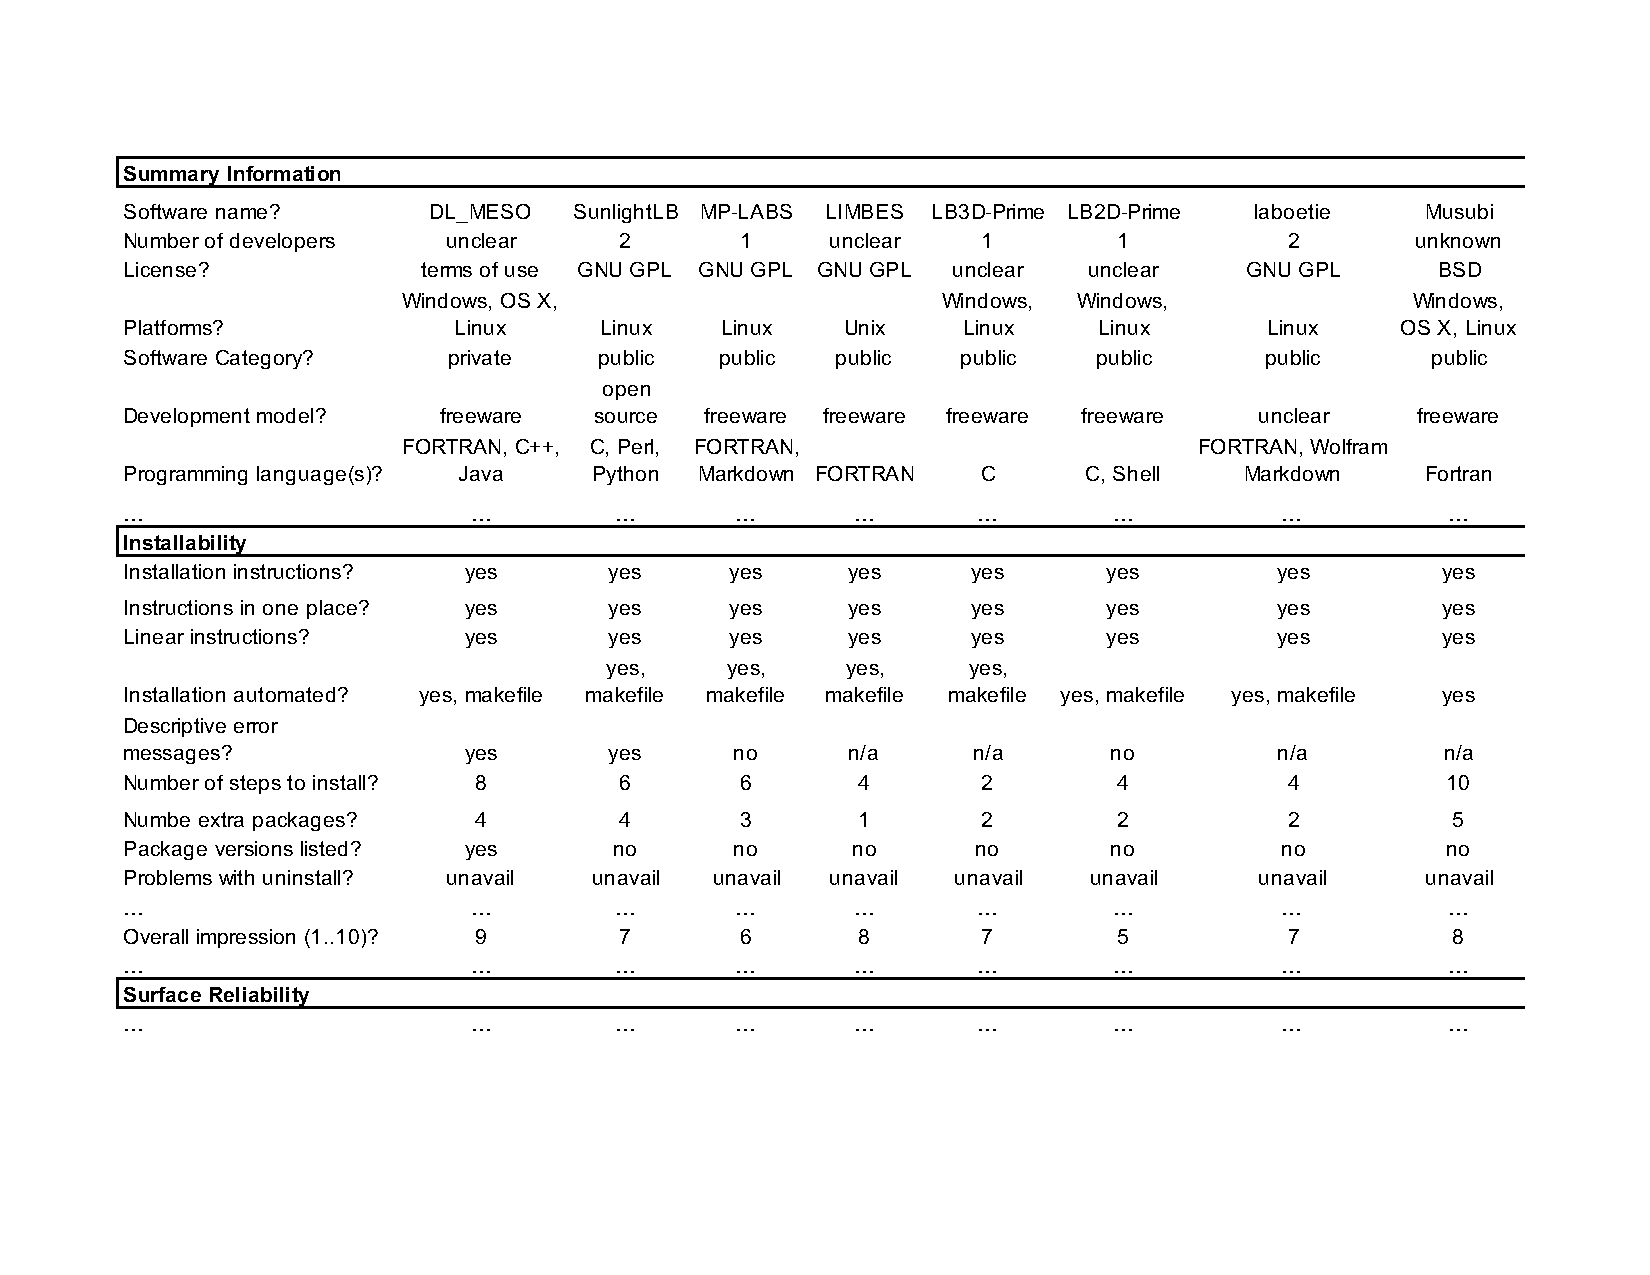
\includegraphics[width=1.0\textwidth]{./figures/measurement_template.pdf}
	  \caption{Excerpt of the Top Sections of the Measurement Template}
	  \label{measurement_template_image}
	\end{center}
\end{figure}

The full template~\cite{SmithEtAl2021} consists of 108 questions categorized
under 9 qualities:
\begin{inparaenum}[(i)]
	\item installability;
	\item correctness and verifiability;
	\item surface reliability;
	\item surface robustness;
	\item surface usability;
	\item maintainability;
	\item reusability;
	\item surface understandability; and,
	\item visibility/transparency. 
\end{inparaenum} 

The questions were designed to be unambiguous, quantifiable and measurable with
limited time and domain knowledge. The measures are grouped under headings for
each quality, and one for summary information
(Figure~\ref{measurement_template_image}).   The summary section provides
general information, such as the software name, number of developers, etc.
Several of the qualities use the word ``surface''.  This is to highlight that,
for these qualities, the best that we can do is a shallow measure. For instance,
we do not conduct experiments to measure usability. Instead, we are looking for
an indication that usability was considered by looking for cues in the
documentation, such as getting started instructions, a user manual or
documentation of expected user characteristics.

Tools are used to find some of the measurements, such as the number of files,
number of lines of code (LOC), percentage of issues that are closed, etc. The
tool \href{https://github.com/tomgi/git_stats}{GitStats} is used to measure
each software package's GitHub repository for the number of binary files, the
number of added and deleted lines, and the number of commits over varying time
intervals. The tool \href{https://github.com/boyter/scc}{Sloc Cloc and Code
(scc)} is used to measure the number of text based files as well as the number
of total, code, comment, and blank lines in each GitHub repository.

Virtual machines (VMs) are used to provide an optimal testing environments for
each package~\cite{SmithEtAl2016} because with a fresh VM there are no worries
about conflicts with existing libraries. Moreover, when the tests are complete
the VM can be deleted, without any impact on the host operating system. The most
significant advantage of using VMs is that every software install starts from a
clean slate, which removes ``works-on-my-computer'' errors.

Once we have measured each package, we still need to rank them to answer
\rqref{RQ_HighestQuality}.  To do this, we used the Analytical Hierarchy Process
(AHP), a decision-making technique that uses pair-wise comparisons to
compare multiple options by multiple criteria \cite{Saaty1980}. In our work AHP
performs a pairwise analysis between each of the 9 quality options for each of
the (approximately) 30 software packages.  This results in a matrix, which is
used to generate an overall score for each software package for the given
criteria~\cite{SmithEtAl2016}.

\begin{figure}[h!]
	\centering
		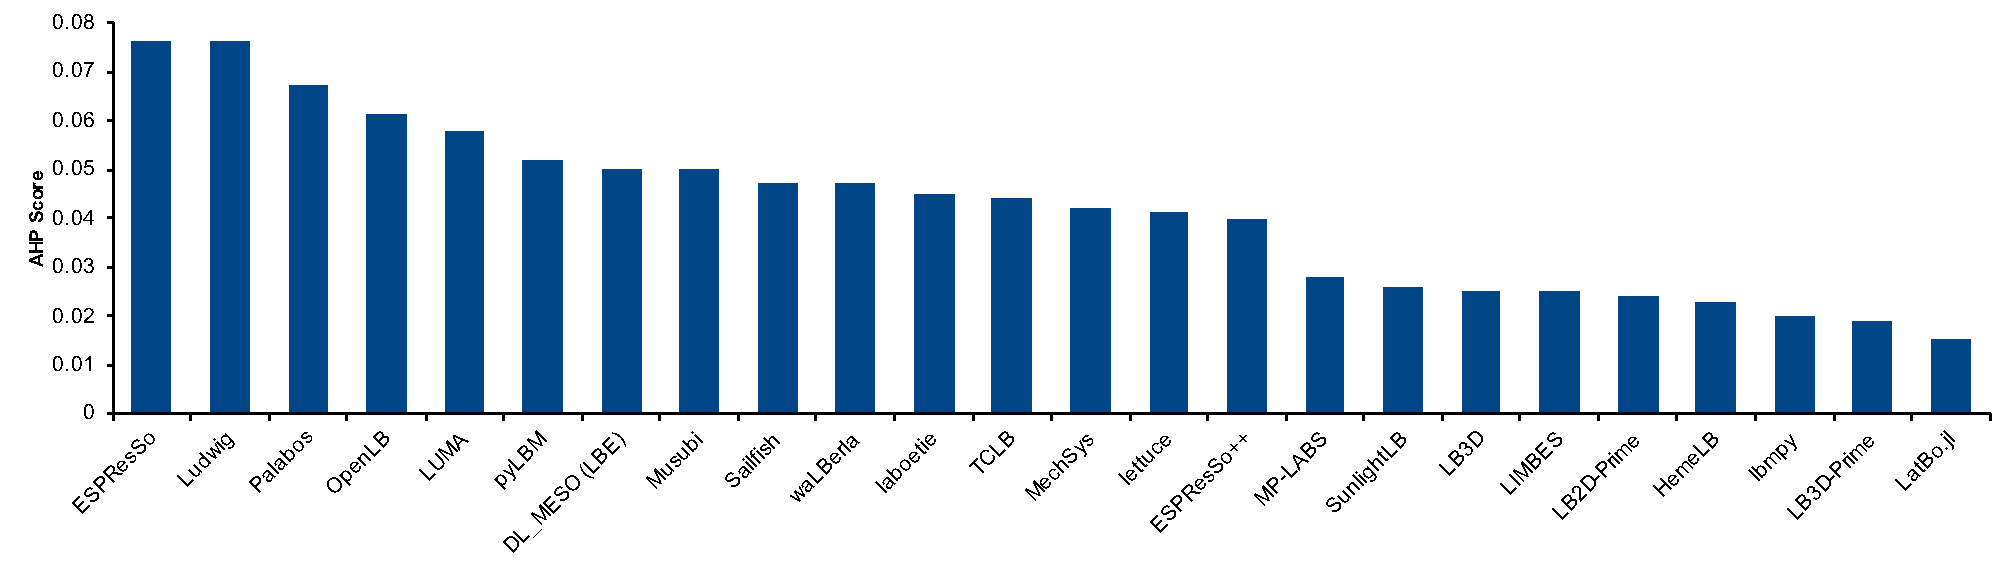
\includegraphics[width=1.0\textwidth]{./figures/finalscore_chart.pdf}
		\caption{AHP Overall Score}
		\label{Fig_OverallScore}
\end{figure}

Figure~\ref{Fig_OverallScore} shows the overall ranking of the LBM software
packages. In the absence of other information on priorities, the overall ranking
was calculated by assuming an equal weighting between all qualities.  The LBM data is available \href{https://github.com/smiths/AIMSS/blob/master/StateOfPractice/DomainMeasurements/LBM-Peter/Completed_LBS_Combined_MeasurementTemplate_EmpiricalMeasures_ADDED_MUSUBI_UPDATED_STATS.xlsx} {on-line}.

\subsection{Interview Developers} \label{SecSurvey}

Several of the research question (\rqref{RQ_CompareToolsProjMngmnt},
\rqref{RQ_CompareMethodologies} and \rqref{RQ_PainPoints}) require going beyond
the quantitative data from the measurement template. To gain the required
insight, we interview developers using a list of 20 questions
\cite{SmithEtAl2021}. The questions cover the background of the development
teams, the interviewees, and the software itself. We ask the developers how they
organize their projects and about their understanding of the users. Some
questions focus on the current and past difficulties, and the solutions the team
has found, or will try. We also discuss the importance of, and the current
situation for, documentation. A few questions are about specific software
qualities, such as maintainability, usability, and reproducibility. The
interviews are semi-structured based on the question list.  Each interview
should take about 1 hour.

The interviewees should follow standard ethics guidelines for consent,
recording, and including participant details in the report. The interview
process presented here was approved by the McMaster University Research Ethics
Board under the application number 
\href{https://github.com/smiths/AIMSS/blob/master/StateOfPractice/MACREM/Application.pdf}
{MREB\#: 5219}.  For LBM we were able to recruit 4 developers to participate in
our study.

\subsection{Interaction With Domain Expert} \label{sec_vet_software_list}

Our methodology relies on engaging a Domain Expert to vet the list of projects
(\rqref{RQ_WhatProjects}) and the AHP ranking (\rqref{RQ_HighestQuality}).  The
Domain Expert is an important member of the assessment
team. Pitfalls exist if non-experts attempt to acquire an authoritative list of
software, or try to definitively rank software. Non-experts have the problem
that they can only rely on information available on-line, which has the
following drawbacks:
\begin{inparaenum}[i)]
  \item the on-line resources could have false or inaccurate information; and,
  \item the on-line resources could leave out relevant information that is so
in-grained with experts that nobody thinks to explicitly record it.
\end{inparaenum}
Domain experts may be recruited from academia or industry.  The only
requirements are knowledge of the domain and a willingness to be involved.

\subsection{Domain Analysis} \label{SecDomainAnalysis}

For the current methodology time constraints necessitate a shallow domain
analysis. For each domain a table should be constructed that distinguishes the
programs under study by their variabilities.  In research software the
variabilities are often assumptions. Table~\ref{tbl_features} shows the
variabilities for LBM software~\cite{Michalski2021}.

\begin{table}[h!]
	\begin{center}
		\begin{tabular}{ p{3cm}p{1.25cm}p{2.25cm}llllll}
			\toprule
			Name & Dim & Pll & Com & Rflx & MFl & Turb & CGE & OS\\
			\midrule
			DL\_MESO (LBE) & 2, 3 & MPI/OMP & Y & Y & Y & Y & Y & W, M, L\\
			ESPResSo & 1, 2, 3 & CUDA/MPI & Y & Y & Y & Y & Y & M, L\\
			ESPResSo++ & 1, 2, 3 & MPI & Y & Y & Y & Y & Y & L\\
			HemeLB & 3 & MPI & Y & Y & Y & Y & Y & L\\
			laboetie & 2, 3 & MPI & Y & Y & Y & Y & Y & L\\
			LatBo.jl & 2, 3 & - & Y & Y & Y & N & Y & L\\
			LB2D-Prime & 2 & MPI & Y & Y & Y & Y & Y & W, L\\
			LB3D & 3 & MPI & N & Y & Y & Y & Y & L\\
			LB3D-Prime & 3 & MPI & Y & Y & Y & Y & Y & W, L\\
			lbmpy & 2, 3 & CUDA & Y & Y & Y & Y & Y & L\\
			lettuce & 2, 3 & CUDA & Y & Y & Y & Y & Y & W, M, L\\
			LIMBES & 2 & OMP & Y & Y & N & N & Y & L\\
			Ludwig & 2, 3 & MPI & Y & Y & Y & Y & Y & L\\
			LUMA & 2, 3 & MPI & Y & Y & Y & Y & Y & W, M, L\\
			MechSys & 2, 3 & - & Y & Y & Y & Y & Y & L\\
			MP-LABS & 2, 3 & MPI/OMP & N & Y & Y & N & N & L\\
			Musubi & 2, 3 & MPI & Y & Y & Y & Y & Y & W, L\\
			OpenLB & 1, 2, 3 & MPI & Y & Y & Y & Y & Y & W, M, L\\
			Palabos & 2, 3 & MPI & Y & Y & Y & Y & Y & W, L\\
			pyLBM & 1, 2, 3 & MPI & Y & Y & N & Y & Y & W, M, L\\
			Sailfish & 2, 3 & CUDA & Y & Y & Y & Y & Y & M, L\\
			SunlightLB & 3 & - & Y & Y & N & N & Y & L\\
			TCLB & 2, 3 & CUDA/MPI & Y & Y & Y & Y & Y & L\\
			waLBerla & 2, 3 & MPI & Y & Y & Y & Y & Y & L\\
			\bottomrule
		\end{tabular}
		\caption{Features of Software Packages (Dim for Dimension (1, 2, 3), Pll
			for Parallel (CUDA, MPI, OpenMP (OMP)), Com for Compressible (Yes or
			No), Rflx for Reflexive Boundary Condition (Yes or No), MFl for
			Multi-fluid (Yes or No), Turb for Turbulent (Yes or No), CGE for
			Complex Geometries (Yes or No), OS for Operating System (Windows
			(W), macOS (M), Linux (L)))} \label{tbl_features}
	\end{center}
\end{table}

\section{Comparison to Community Ranking} \label{repmetrics}

To address \rqref{RQ_CompareHQ2Popular} we need to compare the ranking by best
practices to the community's ranking.  Our best practices ranking comes from the
AHP ranking (Section~\ref{empiricalmeasures}).  We estimate the community's
ranking by repository stars and watches.  The comparison will provide insight on
whether best practices are rewarded by popularity.  However, inconsistencies
between the AHP ranking and the communities ranking are inevitable for the
following reasons: 
\begin{inparaenum}[i)]
	\item the overall quality ranking via AHP makes the unrealistic assumption
	of equal weighting between quality factors;
	\item stars are known to not be a particularly good measure of popularity,
	because of how people use stars and because young projects have less time to
	accumulate stars~\cite{Szulik2017}; 
	\item and, as for consumer products, there are more factors influencing
	popularity than just quality.
\end{inparaenum}

Table~\ref{repometrics} compares the AHP ranking of the LBM package to their
popularity in the research community.  Nine packages do not use GitHub, so they
do not have a measure of stars. Looking at the stars of the other 15 packages,
we can observe a pattern where packages that have been highly ranked by our
assessment tend to have more stars than lower ranked packages. The best ranked
package by AHP (ESPResSo) has the second most stars, while the ninth ranked
package (Sailfish) has the highest number of stars. Although the AHP ranking and
the community popularity estimate are not perfect measures, they do suggest a
correlation between best practices and popularity.

\begin{table}[!h]
	\begin{center}
		\begin{tabular}{ p{3cm}p{1.25cm}p{1.75cm}p{1.75cm}p{1.75cm}p{1.75cm} }
			\toprule
			Name & Our Ranking & Repository Stars & Repository Star Rank &
			Repository Watches & Repository Watch Rank\\
			\midrule
			ESPResSo & 1 & 145 & 2 & 19& 2\\
			Ludwig & 2 & 27 & 8 & 6& 7\\
			Palabos & 3 & 34 & 6 & GitLab& GitLab\\
			OpenLB & 4 & No Git & No Git & No Git& No Git\\
			LUMA & 5 & 33 & 7 & 12& 4\\
			pyLBM & 6 & 95 & 3 & 10& 5\\
			DL\_MESO (LBE) & 7 & No Git & No Git & No Git & No Git\\
			Musubi & 8 & No Git & No Git & No Git & No Git\\
			Sailfish & 9 & 186 & 1 & 41& 1\\
			waLBerla & 10 & 20 & 9 & GitLab& GitLab\\
			laboetie & 11 & 4 & 13 & 5& 8\\
			TCLB & 12 & 95 & 3 & 16& 3\\
			% MechSys & 13 & No Git & No Git & No Git& No Git\\
			% lettuce & 14 & 48 & 4 & 5& 8\\
			% ESPResSo++ & 15 & 35 & 5 & 12& 4\\
			% MP-LABS & 16 & 12 & 11 & 2& 9\\			
			% SunlightLB & 17 & No Git & No Git & No Git& No Git\\
			% LB3D & 18 & No Git & No Git & No Git& No Git\\			
			% LIMBES & 19 & No Git & No Git & No Git& No Git\\
			% LB2D-Prime & 20 & No Git & No Git & No Git& No Git\\		
			% HemeLB & 21 & 12 & 11 & 12& 4\\
			% lbmpy & 22 &  11 & 12 & 2& 9\\	
			% LB3D-Prime & 23 & No Git & No Git & No Git& No Git\\	
			... & ... & ... & ... & ... & ...\\				
			LatBo.jl & 24 & 17 & 10 & 8& 6\\			
			\bottomrule
		\end{tabular}
		\caption{Excerpt from Repository Ranking Metrics~\cite{Michalski2021}}
		\label{repometrics}
	\end{center}
	\end{table}

\section{Comparison of Artifacts to Other Research Software}
\label{Sec_CompareArtifacts}

We answer \rqref{RQ_CompareArtifacts} by comparing the artifacts that we observe
to those observed and recommended for research software in general.  While
filling in the measurement template (Section~\ref{empiricalmeasures}), the
domain software is examined for the presence of artifacts, which are then
categorized by frequency as: common (more than 2/3 of projects), less common
(between 1/3 and 2/3), and rare (less than 1/3). The observed frequency of
artifacts should then be compared to the artifacts recommended by research
software guidelines, as summarized in Table~\ref{Tbl_Guidelines}.  

\begin{table}[!h]
\begin{center}
\begin{tabular}{ p{3cm}p{1cm}p{1cm}p{1cm}p{1cm}p{1cm}p{1cm}p{1cm}p{1cm}p{1cm} }
\toprule
~ \ & \cite{USGS2019} & \cite{TobiasEtAl2018} & \cite{BrettEtAl2021} & \cite{WilsonEtAl2016} & \cite{SmithAndRoscoe2018} & \cite{HerouxEtAl2008} & \cite{ThielEtAl2020} & \cite{vanGompelEtAl2016} & \cite{OrvizEtAl2017}\\
\midrule
LICENSE & \checkmark &  & \checkmark & \checkmark & \checkmark & & \checkmark & \checkmark & \checkmark \\
README &  &  & \checkmark & \checkmark & \checkmark & & \checkmark & \checkmark & \checkmark\\
CONTRIBUTING &  &  & \checkmark & \checkmark & \checkmark & & \checkmark & \checkmark & \checkmark \\
CITATION &  &  &  & \checkmark & & & & \checkmark & \checkmark \\
CHANGELOG &  &  &  & \checkmark & \checkmark & & \checkmark & & \\
INSTALL &  &  &  &  & \checkmark & & \checkmark & \checkmark & \checkmark\\
Uninstall &  &  &  &  & & & & \checkmark & \\
Getting started &  &  &  &  & \checkmark & & \checkmark & \checkmark & \checkmark\\
User manual &  &  & \checkmark &  & & & \checkmark & & \\
Tutorials &  &  &  &  & & & \checkmark & & \\
FAQ &  &  &  &  & & & \checkmark & \checkmark & \checkmark\\
Dependency List &  &  & \checkmark & & \checkmark & & & \checkmark & \\
Issue Track &  & \checkmark & \checkmark & & \checkmark & \checkmark & \checkmark & & \checkmark \\
Version Control &  & \checkmark & \checkmark & \checkmark & \checkmark & \checkmark & \checkmark & \checkmark & \checkmark\\ 
Requirements &  & \checkmark &  & \checkmark & & \checkmark & \checkmark & \checkmark & \checkmark \\
Design &  & \checkmark  & \checkmark &  & \checkmark & & \checkmark & \checkmark& \checkmark\\
API Doc. &  &  &  &  & \checkmark & & \checkmark & \checkmark & \checkmark\\
Build Scripts &  & \checkmark &  & \checkmark & \checkmark & \checkmark & \checkmark & & \checkmark \\
Unit Tests & \checkmark & \checkmark & \checkmark &  & \checkmark & \checkmark & \checkmark & \checkmark & \checkmark \\
Test Plan &  & \checkmark &  &  & & \checkmark & & & \\
Integ. Tests &  & \checkmark & \checkmark &  & & & & \checkmark & \checkmark \\
System Tests &  & \checkmark & \checkmark &  & & \checkmark & & \checkmark & \checkmark \\
Acceptance Tests &  & \checkmark &  &  & & & & &  \\
Regression Tests &  &  & \checkmark &  & & \checkmark & & & \checkmark \\
Code Style Guide &  & \checkmark &  &  & & & \checkmark & \checkmark & \checkmark \\
Release Info. &  & \checkmark &  &  & & \checkmark & \checkmark & & \\
Product Roadmap &  &  &  &  & & \checkmark & \checkmark & \checkmark & \\
Code of Conduct &  &  &  &  & & & \checkmark & & \\
\midrule
\end{tabular}
\caption{Commonly Recommended Artifacts in Software Development Guidelines} \label{Tbl_Guidelines}
\end{center}
\end{table}

The majority of LBM generated artifacts (summarized below) correspond to general
recommendations from research software developers.  For LBM, a union of the
three categories mostly corresponds to general research software recommendations
(Table~\ref{Tbl_Guidelines}). Areas where LBM developers could improve include
providing: API documentation, a roadmap, a code of conduct, programming style
guide, and uninstall instructions.

\begin{description}
	\item[Common:] Developer List, Issue Tracker, Dependency List, Installation
	Guide, Theory Notes, Related Publications, Build Files, README File,
	License, Tutorial, Version Control
	\item[Less Common:] Change Log, Design Doc., Functional Spec., Performance
	Info., Test Cases, User Manual
	\item[Rare:] API Doc., Developer Manual, FAQ, Verification Plan, Video Guide,
	Requirements Spec.
\end{description}

\section{Comparison of Tools to Other Research Software}
\label{Sec_CompareTools}

Software tools are used to support the development, verification, maintenance,
and evolution of software, software processes, and artifacts~\cite[p.\
501]{GhezziEtAl2003}. Development tools support the development of end products,
but do not become part of them, unlike dependencies that remain in the
application once it is released \cite[p.\ 506]{GhezziEtAl2003}. To answer
\rqref{RQ_CompareToolsProjMngmnt} we summarize tools that are visible in the
repositories and that are mentioned during the developer interviews.  As an
example, the tools found for LBM software packages are as follows:

\begin{description}
	\item[Development Tools:] Continuous Integration, Code Editors, Development
	Environments, Runtime Environments, Compilers, Unit Testing Tools,
	Correctness Verification Tools
	\item[Dependencies:] Build Automation Tools, Technical Libraries, Domain
	Specific Libraries
	\item[Project Management Tools:] Collaboration Tools, Email, Change Tracking
	Tools, Version Control Tools, Document Generation Tools
\end{description}

Once the data on tools is collected, the use of two specific tools should be
compared to research software norms: version control and continuous integration.
A little over 10 years ago version control was estimated to be used in only 50\%
of research software projects \cite{Nguyen-HoanEtAl2010}, but even at that time
\cite{Nguyen-HoanEtAl2010} noted an increase from previous usage levels. More
recently, version control usage rates for active mesh generation, geographic
information system and statistical software packages were close to
100\%~\cite{Smith2018}.  Almost every software guide cited in
Table~\ref{Tbl_Guidelines} includes the advice to use version control. For LBM
packages 67\% use version control (GitHub, GitLab or CVS). The high usage of
version control tools in LBM software matches the trend in research software in
general.

Continuous integration is rarely used in LBM (3 of 24 packages or 12.5\%). This
contrasts with the frequency with which continuous integration is recommended in
research software development
guidelines~\cite{BrettEtAl2021,vanGompelEtAl2016,ThielEtAl2020}. In this case,
it seems likely that the recommendations are ahead of common practice.

\section{Comparison of Processes to Other Research Software} \label{Sec_CompareMethodologies}

The interview data on development processes is used to answer research question
\rqref{RQ_CompareMethodologies}.  This data should be contrasted with the
development process used by research software in general. The literature
suggests that scientific developers naturally use an agile philosophy
\cite{CarverEtAl2007,Segal2005}, or an amethododical process \cite{Kelly2013}.
Another point of comparison should be on the use of peer review, since peer
review is frequently recommended~\cite{HerouxEtAl2008,OrvizEtAl2017,USGS2019}.

The LBM example confirms an informal, agile-like, process. The development
process is not explicitly indicated in the artifacts. However, during interviews
one developer (ESPResSo) told us their non-rigorous development model is like a
combination of agile and waterfall. Employing a loosely defined process makes
sense for LBM software, given that the teams are generally small and
self-contained. One of the developers (ESPResSo) also noted that they use an ad
hoc peer review process.

\section{Developer Pain Points} \label{painpoints}

To answer \rqref{RQ_PainPoints}, we ask developers about their pain points and
compare their responses to the literature~\cite{WieseEtAl2019,PintoEtAl2018}.
Pain points to watch for include: cross-platform compatibility, scope bloat,
lack of user feedback, dependency management, data handling concerns,
reproducibility, and software scope. 

An example pain point noted for LBM is a lack of development time. A developer
of pyLBM noted that their small development team did not have enough time to
implement new features. Small development teams are common for LBM software
packages (as shown in Figure~\ref{measurement_template_image}).

\section{Threats To Validity} \label{threats}

The measures in the measurement template~\cite{SmithEtAl2021} may not be broad
enough to accurately capture some qualities. For example, there are only two
measures of surface robustness. Similarly, reusability is assessed by the number
of code files and LOC per file, assuming that a large number of relatively small
files implies modularity. Furthermore, the measurement of understandability
relies on 10 random source code files. It is possible that the 10 files that
were chosen to represent a software package may not be a good representation.

Another risk to the validity of the proposed approach is missing or incorrect
data. Some software package data may not have been measured due to technology
issues like broken links. For the LBM example, this issue arose with the
measurement of Palabos, which had a broken link to its user manual. Some
pertinent data may not have been specified in public artifacts, or may be
obscure within an artifact or web-page. For the LBM example, the use of unit
testing and continuous integration was mentioned in the artifacts of only three
(ESPResSo, Ludwig, Musubi) packages. However, interviews suggested a more
frequent use of both unit testing and continuous integration in the development
processes.

\section{Concluding Remarks} \label{SecConcludingRemarks}

To improve the development of research software, both in terms of productivity,
and the resulting software quality, we need to understand the current state of
the practice. An exciting strategy to approach this goal is to assess one domain
at a time, collecting data from developer interviews and digging deeply into
their code repositories. By providing feedback specific to their domain, the
developer community can be drawn into a dialogue on how to best make
improvements going forward. Moreover, they can be encouraged to share their best
practices between one another, and with other research software domains.

We have outlined a methodology for assessing the state of the practice for any
given research software domain based on a list of about 30 representative
projects.  In addition to interviews, we use manual and automated inspection of
the artifacts in each project's repositories.  The repository data is collected
by filling in a 108 question measurement template, which requires installing the
software on a VM, running simple tests (like completing the getting started
instructions (if present)), and searching the code, documentation and test
files. Using AHP the projects are ranked for 9 individual qualities
(installability, correctness and verifiability, reliability, robustness,
usability, maintainability, reusability, surface understandability,
visibility/transparency) and for overall quality.  Perspective and insight is
shared with the user community via the following: i) comparing the ranking by
best practices against an estimate of the communities ranking of popularity; ii)
comparing artifacts, tools and processes to current research software
development guidelines; and, iii) exploring pain points via developer
interviews. Using our methodology, spreadsheet templates and AHP tool, we
estimate (based on our experience with using the process) the time to complete
an assessment for a given domain at 173 person hours.

For the running example of LBM we found that the top packages engaged in most of
recommended best practices, including examples of practising peer review.
However, we did find room for improvement with respect to providing API
documentation, a roadmap, a code of conduct, programming style guide, and
uninstall instructions.  In addition, the community could likely benefit by
increased use of continuous integration.

Building from the LBM example we can create a wealth of data on multiple
domains.  The next step is a meta-analysis, where we look at how the different
domains compare to answer new research questions like: What lessons from one
domain could be applied in other domains? What (if any) differences exist in the
pain points between domains?  Are there differences in the tools, processes, and
documentation between domains?

%
% ---- Bibliography ----
%
% BibTeX users should specify bibliography style 'splncs04'.
% References will then be sorted and formatted in the correct style.
%
\bibliographystyle{splncs04}
\bibliography{DiggingDeeper}
%
% \begin{thebibliography}{8}
% \bibitem{ref_article1}
% Author, F.: Article title. Journal \textbf{2}(5), 99--110 (2016)

% \bibitem{ref_lncs1}
% Author, F., Author, S.: Title of a proceedings paper. In: Editor,
% F., Editor, S. (eds.) CONFERENCE 2016, LNCS, vol. 9999, pp. 1--13.
% Springer, Heidelberg (2016). \doi{10.10007/1234567890}

% \bibitem{ref_book1}
% Author, F., Author, S., Author, T.: Book title. 2nd edn. Publisher,
% Location (1999)

% \bibitem{ref_proc1}
% Author, A.-B.: Contribution title. In: 9th International Proceedings
% on Proceedings, pp. 1--2. Publisher, Location (2010)

% \bibitem{ref_url1}
% LNCS Homepage, \url{http://www.springer.com/lncs}. Last accessed 4
% Oct 2017
% \end{thebibliography}

\end{document}